\section{Approach} 
\label{approach}

% Research question
Our epistemic research interest is to clarify the question, whether classical Machine Learning methods combined with suitable features can outperform neural network based approaches.

Figure \ref{fig:overall_pipeline} visualizes our approach (on the top) and the resulting novelties achieved through our work (at the bottom). The following chapters describe the different steps in detail. First the data is preprocessed (chapter \ref{ch:approachA}, \ref{ch:approachB}). 
The next step differs between classical Machine Learning methods and neural network based approaches. For classical Machine Learning methods an explicit feature extraction is necessary. Due to the fact that our dataset unbalanced, we further create an unbalanced, oversampled and undersampled datasets (chapter \ref{ch:approachD}). Finally the classifiers are trained, evaluated and the results are compared (chapter \ref{ch:approachE}, \ref{ch:approachF}). 

\begin{figure}[ht]
	\centering
	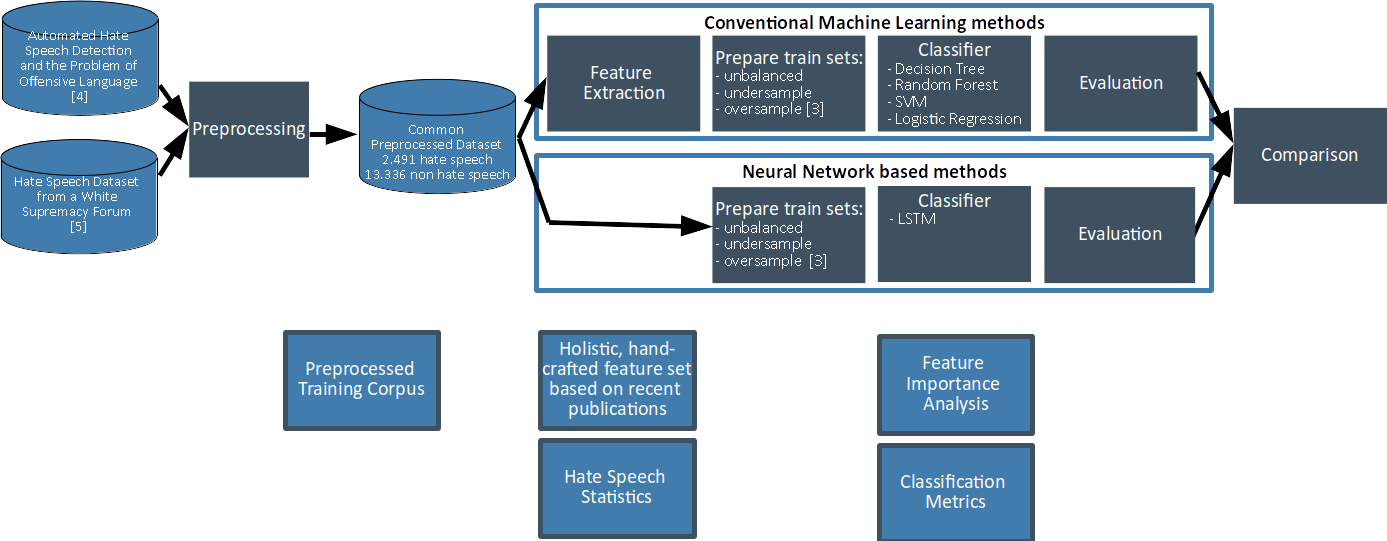
\includegraphics[width=1.0\linewidth]{figures/pipeline.png}
	\caption{Approach}
	\label{fig:overall_pipeline}
\end{figure}

\subsection{Definition of Hate Speech} 
\label{ch:approachA}

\subsection{Preprocessing}
\label{ch:approachB}

\subsection{Features}
\label{ch:approachC}

For the conventional Machine Learning methods we built a hand-crafted feature set. The selection of features is based on recent works \cite{Watanabe2018} and \cite{Fortuna2018}. In the following the feature groups, the extraction process and the evaluation approach for the feature importances are introduced.

\subsubsection*{Feature groups}

Our feature set consists of features from the following five groups:
\begin{itemize}
	\item Unigram features \cite{ThomasDavidson2020, Fortuna2018, Gaydhani2018, Malmasi2017, Oriola2020}
	\begin{itemize}
		\item N-grams
		\item Dictionaries based on TF-IDF
	\end{itemize}
	\item Semantic features \cite{ThomasDavidson2020, Watanabe2018}
	\begin{itemize}
		\item Number of exclamation/question/full stop marks
		\item Number of capitalized words
		\item Number of laughing expressions
	\end{itemize}
	\item Pattern features \cite{Fortuna2018, Oriola2020}
	\begin{itemize}
		\item PoS-tag patterns
	\end{itemize}
	\item Topic classification \cite{Fortuna2018}
	\begin{itemize}
		\item Latent Dirichlet Allocation
	\end{itemize}
	\item Sentiment-based features \cite{Fortuna2018, Oriola2020}
	\begin{itemize}
		\item Polarity scores based on Vader
	\end{itemize}
\end{itemize}

\subsubsection*{Feature extraction}
% Reusable pipeline
The feature extraction of the previously mentioned features is done within a reusable pipeline, which makes it easy to add new features. Each feature is implemented as a class following a predefined structure. By adding the feature class to a list in the Feature\-Extractor the feature is automatically extracted as part of the pipeline. The pipelines input are the data instances as text and the output is a dataframe containing all extracted features as numerical values.

\subsubsection*{Feature importances}
% Feature importances


\subsection{Dataset}
\label{ch:approachD}

TODO: Intro

Depending on the method the inputs vary. For the classical Machine Learning methods the inputs are the extracted features as numerical values, whereas in neural network based approaches the inputs are the raw textual features. The labels are in both cases numerical values.

Then we perform the dataset balancing.
TODO: Dataset balancing


Finally we receive unbalanced, undersampled and oversampled datasets.

TODO: name that oversampling currently not present for nn approaches


\subsection{Classifiers}
\label{ch:approachE}

This chapter deals with the classifiers and their integration into the project.

Each classifier is trained on the training set and evaluated on the test set. So the same steps are necessary for each classifier. That is why a reusable pipeline is developed. The pipeline is developed with the Open Closed principle in mind. It is open for extensions and closed for changes. So when adding a new classifier only a few lines of code need to be adapted and steps such as finding the optimal model through hyperparameter tuning and the evaluation are done automatically as part of the pipeline.

As the methods need it, there are slight differences between the training of the classical Machine Learning methods and the neural network based approaches. Figure \ref{fig:classifier_pipeline} illustrates this.

\begin{figure}[ht]
	\centering
	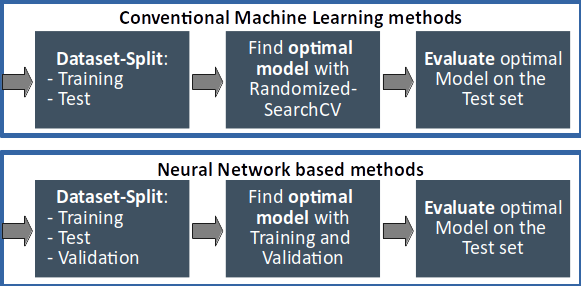
\includegraphics[width=0.7\linewidth]{figures/classifier_pipeline.png}
	\caption{Classifier pipeline}
	\label{fig:classifier_pipeline}
\end{figure}

For the classical Machine Learning methods the dataset is split into training (0.8) and test set (0.2). For finding the optimal model Randomized\-SearchCV is executed on the defined hyperparameter search space. The hyperparameter search space was chosen based on the classifiers doc\-u\-men\-ta\-tion, papers and by an empirical examination. For the decision tree \cite{mantovani2019empirical} and for the random forest \cite{probstHyperparametersTuningStrategies2019} were observed. Finally the model is evaluated on the test set.

TODO: Description for LR, SVM how is the hyperparameter search space set?

For neural network based approaches the dataset is again split into training (0.8) and test set (0.2). Then the training set is further split up into training (0.8) and validation (0.2). In the next step the optimal model is found by using the training and the validation set. The final step is equal to the final step in classical Machine Learning, were the model is evaluated.

To enable a performant execution we use Pythons multiprocessing library to parallelize the execution.

In this work we compare five classifiers on the different datasets (unbalanced, undersampled, oversampled). Four of them are classical Machine Learning methods (Decision Tree, Random Forest, SVM, Logistic Regression) and one neural network based approach (LSTM).


\subsection{Evaluation}
\label{ch:approachF}

For evaluating the classifiers standard metrics such as accuracy, precision, recall and F1 score are used.

The accuracy specifies how many data instances are correctly classified. Only looking at the accuracy, is not that informative, because generally lots of instances are correctly classified as non hate speech, which leads to a high accuracy.

That is why also precision and recall are observed. Precision specifies how many of the predicted hate speech instances are really hate speech. A low precision means that there are lots of instances classified as hate speech, although they are not. So looking at the precision enables to detect if the trained model could built a censoring system and undermine the freedom of speech. The recall specifies how many hate speech instances are correctly classified by the model. A low recall means that there are lots of false negatives (lots of hate speech instances are not detected).

For taking into account precision and recall one can look at the F1 score. 

